\documentclass{article} % For LaTeX2e
\usepackage{nips12submit_e,times}
%\documentstyle[nips12submit_09,times,art10]{article} % For LaTeX 2.09

%% \usepackage{times}
%% \usepackage{epsfig}
\usepackage{graphicx,url,amsmath}
%% \usepackage{amsmath}
%% \usepackage{amssymb}
%% \usepackage{algorithm,algorithmic,setspace}
%% \usepackage{fmtcount}

%% Rob's equation stuff
%% \def\BE{\vspace{-2.0mm}\begin{equation}}
%% \def\EE{\vspace{-1.4mm}\end{equation}}
\def\BE{\vspace{-0.0mm}\begin{equation}}
\def\EE{\vspace{-0.0mm}\end{equation}}

\def\BEA{\vspace{-0.0mm}\begin{eqnarray}}
\def\EEA{\vspace{-0.0mm}\end{eqnarray}}


\newcommand{\ldl}{$\ell_1 / \ell_2$\,}
\newcommand{\lzero}{$\ell_0$\,}
\newcommand{\lone}{$\ell_1$\,}
\newcommand{\ltwo}{$\ell_2$\,}
%\newcommand{\conv}{\otimes}
\newcommand{\conv}{*}

\newcommand{\alg}[1]{Algorithm \ref{alg:#1}}
\newcommand{\eqn}[1]{Eqn.~\ref{eqn:#1}}
\newcommand{\fig}[1]{Fig.~\ref{fig:#1}}
\newcommand{\tab}[1]{Table~\ref{tab:#1}}
\newcommand{\secc}[1]{Section~\ref{sec:#1}}
\def\etal{{\textit{et~al.~}}}

\newcommand{\matt}[1]{\textbf{\textcolor{blue}{#1}}}
\newcommand{\rob}[1]{\textbf{\textcolor{red}{#1}}}



%\title{Stochastic Pooling to Prevent Overfitting in Deep Convolutional Networks}
%\title{Regularization of Convolutional Neural Networks with Stochastic
%  Pooling}
\title{Stochastic Pooling for Regularization of \\ Deep Convolutional Neural Networks}
%% \thanks{ Use footnote for providing further information
%% about author (webpage, alternative address)---\emph{not} for acknowledging
%% funding agencies.}


\author{
Matthew D. Zeiler \\
Department of Computer Science \\
Courant Institute, New York University \\
\texttt{zeiler@cs.nyu.edu} \\
\And
Rob Fergus \\
Department of Computer Science \\
Courant Institute, New York University \\
\texttt{fergus@cs.nyu.edu} \\
}

% The \author macro works with any number of authors. There are two commands
% used to separate the names and addresses of multiple authors: \And and \AND.
%
% Using \And between authors leaves it to \LaTeX{} to determine where to break
% the lines. Using \AND forces a linebreak at that point. So, if \LaTeX{}
% puts 3 of 4 authors names on the first line, and the last on the second
% line, try using \AND instead of \And before the third author name.

\newcommand{\fix}{\marginpar{FIX}}
\newcommand{\new}{\marginpar{NEW}}

\nipsfinalcopy % Uncomment for camera-ready version

\begin{document}


\maketitle

\begin{abstract}
  We introduce a simple and effective method for regularizing large
  convolutional neural networks. We replace the conventional
  deterministic pooling operations with a stochastic procedure,
  randomly picking the activation within each pooling region according
  to a multinomial distribution, given by the activities within the
  pooling region. The approach is hyper-parameter free and can be
  combined with other regularization approaches, such as dropout and
  data augmentation. We achieve state-of-the-art performance on four
  image datasets, relative to other approaches that do not utilize
  data augmentation.
\end{abstract}

\section{Introduction}

Neural network models are prone to over-fitting due to their high
capacity. A range of regularization techniques are used to prevent
this, such as weight decay, weight tying and the augmentation of the
training set with transformed copies \cite{NNtricks}. These allow the
training of larger capacity models than would otherwise be possible,
which yield superior test performance compared to smaller un-regularized models.

Dropout, recently proposed by Hinton \etal \cite{Hinton12}, is another
regularization approach that stochastically sets half the activations
within a layer to zero for each training sample during training. It
has been shown to deliver significant gains in performance across a
wide range of problems, although the reasons for its efficacy are not
yet fully understood.

A drawback to dropout is that it does not seem to have the same
benefits for convolutional layers, which are common in many networks
designed for vision tasks.  In this paper, we propose a novel type of
regularization for convolutional layers that enables the training of
larger models without over-fitting, and produces superior performance
on recognition tasks.

The key idea is to make the pooling that occurs in each convolutional
layer a stochastic process. Conventional forms of pooling such as
average and max are deterministic, the latter selecting the largest
activation in each pooling region. In our stochastic pooling, the
selected activation is drawn from a multinomial distribution
formed by the activations within the pooling region.

An alternate view of stochastic pooling is that it is equivalent to
standard max pooling but with many copies of an input image, each
having small local deformations. This is similar to explicit elastic
deformations of the input images \cite{Simard03}, which delivers
excellent MNIST performance. Other types of data augmentation, such as
flipping and cropping differ in that they are global image
transformations. Furthermore, using stochastic pooling in a
multi-layer model gives an exponential number of deformations since
the selections in higher layers are independent of those below.

%Do you mean dependent or independent above?
%
%Elastic Distortions
%Jitter
%Adding White Noise

\section{Review of Convolutional Networks}

Our stochastic pooling scheme is designed for use in a standard
convolutional neural network architecture. We first review this model,
along with conventional pooling schemes, before introducing our novel
stochastic pooling approach.

A classical convolutional network is composed of alternating layers of
convolution and pooling (i.e.~subsampling).  The aim of the first
convolutional layer is to extract patterns found within local regions
of the input images that are common throughout the dataset.  This is
done by convolving a template or filter over the input image pixels,
computing the inner product of the template at every location in the
image and outputting this as a feature map $c$, for each filter in the
layer. This output is a measure of how well the template matches each
portion of the image. A non-linear function $f()$ is then applied
element-wise to each feature map $c$: $a = f(c)$. The resulting
activations $a$ are then passed to the pooling layer. This aggregates
the information within a set of small local regions, $R$, producing a
pooled feature map $s$ (of smaller size) as output. Denoting the
aggregation function as $pool()$, for each feature map $c$ we have:
\BE s_j = pool(f(c_i)) \;\;\; \forall i \in R_j \EE where $R_j$ is
pooling region $j$ in feature map $c$ and $i$ is the index of each
element within it.

The motivation behind pooling is that the activations in the pooled map
$s$ are less sensitive to the precise locations of structures within
the image than the original feature map $c$. In a multi-layer model,
the convolutional layers, which take the pooled maps as input,
can thus extract features that are increasingly invariant to local
transformations of the input image. This is important for
classification tasks, since these transformations obfuscate the object
identity.

A range of functions can be used for $f()$, with $tanh()$ and logistic
functions being popular choices. In this is paper we use a linear rectification
function $f(c) = max(0,c)$ as the non-linearity. In
general, this has been shown \cite{Nair10} to have significant
benefits over $tanh()$ or logistic functions. However, it is especially
suited to our pooling mechanism since: (i) our formulation involves the non-negativity
of elements in the pooling regions and (ii) the clipping of negative
responses introduces zeros into the pooling regions, ensuring that the
stochastic sampling is selecting from a few specific locations (those
with strong responses), rather than all possible locations in the
region.

There are two conventional choices for $pool()$: average and max. The
former takes the arithmetic mean of the elements in each pooling
region:
\BE s_j = \frac{1}{|R_j|} \sum_{i \in R_j} a_i \:\:\:  \EE
while the max operation selects the largest element:
\BE s_j = \max_{i \in R_j} a_i
\EE

% 1) Only when the
% input region correponding to a given element matches the convolutional
% filters well does an activation get output. This prevents small
% correlations or negative correlations from being passed up to higher
% layers. 2) Positive activations are linear, allowing deep networks to
% be trained without the vanishing gradient problems that occur with
% saturating nonlinearities such as tanh or logistics. Additionally, the
% small or negative feature maps element introduce zeros into the
% forward and back-propagation of the network, helping the network
% become sparse and quickly learn interesting filters. 3) Since the
% nonlinearity does not saturate, perfect correlations are
% proportionally better than near perfrect matches. NOT SURE IF THIS IS
% REALLY RELEVANT.




%The form of the aggregation used  in the feature maps by the following
%pooling layer.  How the feature map elements in the pooling regions
%are aggreated through some form of pooling function which we denote as
%$pool()$. This takes all the feature maps responses within the pooling
%region and produces a single pooled activation, $s$, for the region:
%
%\BE p_j = pool(c_i) \;\;\; \forall i \in R_j \EE where $j$ is the
%index of the pooling region $R_j$ within the overall maps, and $i$ is
%the index of each element in pooling region $R_j$. The goal of this
%pooling layer is to make the represetntation that will subsequently be
%passed on to higher layers more robust to precise locations of the
%lower convolutional templates within the image.


%Adding an additional pair of convolution and pooling layers on top
%proceeds by connecting the next convolutional layer to the pooled
%feature maps. Again this convolution layer will filter the pooled
%feature maps that are output from the first layer and attempt to find
%patterms in these throughout the dataset. As this process proceeds in
%a feedforwad fashion up the network, the convolution filters extract
%more and more abstract patterns made up of lower level feature
%activations. The pooling in higher layers continues to make the
%network more robust to the precise location of these complex patterns
%found in the image.

% Neural-network also

% One additional component of convolutional networks that is an
% important consideration in this paper is nonlinearities throughout the
% network. Typically element-wise nonlinearities such as tanh, logistic,
% or rectified linear units are placed either before or after the
% pooling layers. This allows the overall network to learn nonlinear
% mappings from the input image to the output labels. In this paper we
% utilize rectified linear units \cite{Nair10} between the convolution
% feautre maps $c$ and the input to the pooling layer. We refer to these
% pooling layer inputs as feature activations, $a$, throughout the
% remainder of the text:

% \BE
% a = \max(0,c)
% \EE

% This simple nonlinearity has many nice properties. 1) Only when the
% input region correponding to a given element matches the convolutional
% filters well does an activation get output. This prevents small
% correlations or negative correlations from being passed up to higher
% layers. 2) Positive activations are linear, allowing deep networks to
% be trained without the vanishing gradient problems that occur with
% saturating nonlinearities such as tanh or logistics. Additionally, the
% small or negative feature maps element introduce zeros into the
% forward and back-propagation of the network, helping the network
% become sparse and quickly learn interesting filters. 3) Since the
% nonlinearity does not saturate, perfect correlations are
% proportionally better than near perfrect matches. All these properties
% are important for our proposed pooing mechanism.

% \subsection{Existing Pooling Methods}

% Amongst other hyperparameters such as the number of feature maps in
% convolutional layers and the size of the pooling regions, $N$, is the
% choice of pooling function to use. Typically max or average pooling is
% used to summarize the activations in a pooling region. In the case of
% average pooling, the nonlinear activations in a region are summed and
% divided by the size of the region: \BE p_j = \frac{1}{N} \sum_{i \in
%   R_j} a_j \EE

% In the case of max pooling, the maximum activation within the region
% is chosen as the pooled activation : \BE p_j = \max_{i \in R_j} a_j
% \EE

Both types of pooling have drawbacks when training deep convolutional
networks. In average pooling, all elements in a pooling region are considered,
even if many have low magnitude. When combined with linear rectification
non-linearities, this has the effect of down-weighting strong
activations since many zero elements are included in the average.
Even worse, with $tanh()$ non-linearities, strong positive and negative activations
can cancel each other out, leading to small pooled responses.

While max pooling does not suffer from these drawbacks, we find it easily overfits the training set
in practice,
making it hard to generalize well to test examples. Our proposed pooling scheme has the
advantages of max pooling but its stochastic nature helps prevent
over-fitting.




% There are some small subleties in both types of pooling that can be
% seen as a drawbacks in training deep convolutional networks. In terms
% of average pooling, all elements in a pooling region are considered,
% even if many of the locations of the convolutional filters had little
% or no correlation with the input. When rectified linear nonlinearities
% are used this has the effect of down-weighting strong activations by
% averaging in all the zero elements within the pooling region. Even
% worse, with other types of nonlinearity that preserves negatives, such
% as tanh, averaging elements in a pooling region can simply cancel
% positives and negatives leading to minimal output despite potentially
% large convolution responses.

% These drawbacks of average pooling do no exist in max pooling. Since
% only the maximum element is taken in the region, only strong
% correlations are passed to the next layer and none of the small or
% negative correlations are considered. Max pooling also has the nice
% property of introducing additional sparsity into the gradients helping
% many convolutional architectures learn interesting featurs
% \cite{Zeiler11}.

% We found in practice a network with max pooling to learn much faster
% than with average pooling. This could potentially be due to average
% pooling downwaiting strong activation or max pooling introducing many
% zeros into the backpopagation. While speeding up training by using max
% pooling is good, the trade off is that it can drastically overfit the
% training set. Once the training set accuracy reaches 100\% it is often
% difficult to generalize well to new data. This is where our approach
% comes in.

\section{Stochastic Pooling}

In stochastic pooling, we select the pooled map response by sampling
from a multinomial distribution formed from the activations of each
pooling region. More precisely, we first compute the probabilities $p$
for each region $j$ by normalizing the activations within the
region:
\BE
p_i = \frac{a_i}{\sum_{k \in R_j} a_k}
\label{eqn:multinomial}
\EE

We then sample from the multinomial distribution based on
$p$ to pick a location $l$ within the region. The pooled activation is
then simply $a_l$:
\BE
 s_j = a_l \:\:\: \text{where} \:\: l \sim P(p_1,\ldots,p_{|R_j|})
\EE
The procedure is illustrated in \fig{toy}. The samples for each
pooling region in each layer for each training example are drawn
independently to one another. When back-propagating through the network
this same selected location $l$ is used to direct the gradient back
through the pooling region, analogous to back-propagation with max pooling.

% Given a pooling region $R$ with input activations $a$ we first compute
% a probability $p(i)$ for each element $i$ in the region: \BE p(i) =
% \frac{a_i}{\sum_{k \in R} a_k} \EE

% Given these probabilities we sample from the multinomial distribution
% over postion within the pooling region in order to select a single
% location to use for pooling. Once the location $l$ is chosen, the
% activation at that location $a_l$ is used as the pooled element: \BE p
% = a_l ,\;\;\; where \; l \; is\; sampled \; from\; p(i) \EE

% When backpropagating through the network this same selected location
% $l$ is used to direct the gradient back through the pooling region, analagous to
% backpropagation with max pooling. The rectified linear
% nonlinearity ensures that many of the
% probabilities $p(i)$ will be zero, leaving probability mass only on
% the remaining activations, proportional to their strength. Higher
% probability is naturally given to locations that match the input
% patter better. In expectation, while sampling locations each time an
% image is visited, the stronger activations will be used proportionally
% more than weaker activations, however these weak ativations still have
% a role unlike in max pooling.


% The toy example in \fig{toy} shows how this stochastic selection of
% the element to use can capture more information about the pooling
% region than either max or average pooling. In expectation any input
% distribution could be modelled throughout training. This is done while
% maintaining all of the benefits of max pooling such as sparsity in the
% gradients which leads to fast training and avoiding the drawbacks of
% average pooling such as downwaiting strong activations.

Max pooling only captures the strongest activation of the filter
template with the input for each region. However, there may be
additional activations in the same pooling region that should be taken
into account when passing information up the network and stochastic
pooling ensures that these non-maximal activations will also be utilized.


% ultimately to the classifier. Stochastic
% pooling allows  As we have
% seen averaging is not adequate as it incorporaes the element in the
% pooling region where little or no correlation existed. To incorporate
% more than one element we propose a sampling proceedure which considers
% all elements in a pooling region as candidates.

\begin{figure}[h!]
\begin{center}
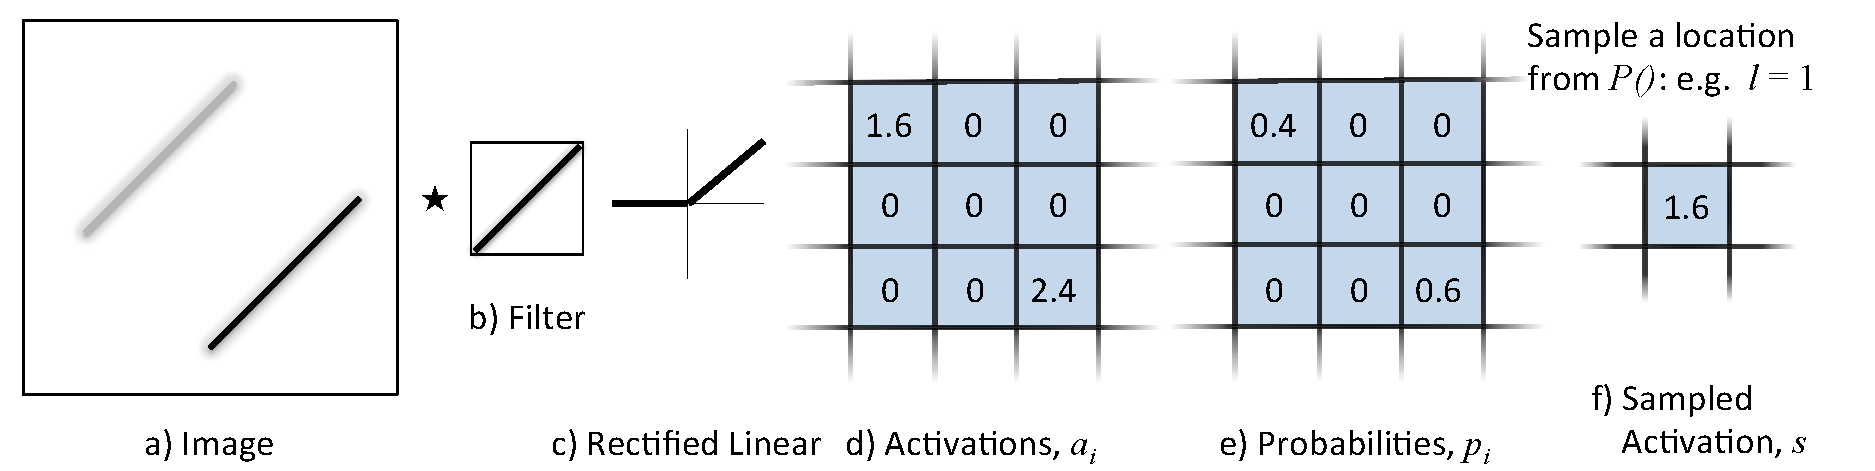
\includegraphics[width=5.5in]{toy.pdf}
\end{center}
\vspace*{-0.2cm}
\caption{Toy example illustrating stochastic pooling. a) Input image. b)
  Convolutional filter. c) Rectified linear function. d) Resulting activations within a given pooling region. e) Probabilities based
  on the activations. f) Sampled activation. Note that the selected
  element for the pooling region may not be the largest
  element. Stochastic pooling can thus represent multi-modal
  distributions of activations within a region.}
\label{fig:toy}
\vspace*{-0.2cm}
\end{figure}


\subsection{Probabilistic Weighting at Test Time}

Using stochastic pooling at test time introduces noise into
the network's predictions which we found to degrade performance (see \secc{averaging}). Instead, we
use a probabilistic form of averaging. In this, the activations in
each region are weighted by the probability $p_i$ (see
\eqn{multinomial}) and summed:
\BE
s_j = \sum_{i \in R_j} p_i a_i
\EE
This differs from standard average pooling because each element has a potentially different
weighting and the denominator is the
sum of activations $\sum_{i \in R_j} a_i$, rather than the pooling
region size $|R_j|$. In practice, using conventional average (or sum) pooling
results in a huge performance drop (see \secc{averaging}).


% At test time we found that sampling a new location added too much
% noise to the prediction. While this is good for training, this hurts
% classification performance as shown in section
% \secc{averaging}. Instead we propose to instead use the probabilities
% over a pooling region to do a weighted sum of the input elements. This
% gives more weight to the stronger activations, less weight to weak
% activations, and zero weight negative or no correlation existed. This
% significantly improves classification performance at test time.

Our probabilistic weighting can be viewed as a form of model averaging
in which each setting of the locations $l$ in the pooling regions
defines a new model. At training time, sampling to get new locations
produces a new model since the connection structure throughout the
network is modified. At test time, using the probabilities instead of
sampling, we effectively get an estimate of averaging over all of these possible
models without having to instantiate them.
Given a network architecture with $d$ different pooling
regions, each of size $n$, the number of possible models is $n^d$ where $d$ can be in
the $10^4$-$10^6$ range and $n$ is typically 4,9, or 16 for example
(corresponding to $2\times2$, $3\times3$ or $4\times4$ pooling
regions). This is a significantly larger number than the model averaging
that occurs in dropout \cite{Hinton12}, where $n=2$ always (since an activation is either present or
not).
In \secc{averaging} we confirm that using this
probability weighting achieves similar performance compared to using a large number of model
instantiations, while requiring only one pass through the network.

Using the probabilities for sampling at training time and for
weighting the activations at test time leads to state-of-the-art
performance on many common benchmarks, as we now demonstrate.

\section{Experiments}
\label{exp_sec}

\subsection{Overview}
We compare our method to average and max pooling on a
variety of image classification tasks. In all experiments we use
mini-batch gradient descent with momentum to optimize the cross
entropy between our network's prediction of the class and the ground
truth labels. For a given parameter $x$ at time $t$ the weight updates
added to the parameters, $\Delta x_t$ are $\Delta x_t = 0.9 \Delta
x_{t-1} - \epsilon g_t$ where $g_t$ is the gradient of the cost
function with respect to that parameter at time $t$ averaged over the
batch and $\epsilon$ is a learning rate set by hand.

All experiments were conducted using an extremely efficient C++ GPU
convolution library \cite{cudaconvnet} wrapped in MATLAB using GPUmat
\cite{gpumat}, which allowed for rapid development and
experimentation. We begin with the same network layout as in Hinton
\etal's dropout work \cite{Hinton12}, which has $3$ convolutional layers
with 5x5 filters and $64$ feature maps per layer with rectified linear units as their
outputs. We use this same model and train for 280 epochs in all experiments aside
from one additional model in \secc{SVHN} that has 128 feature maps in layer 3 and is trained for 500
epochs. Unless otherwise specified we use $3 \times 3$
pooling with stride $2$
(i.e.~neighboring pooling regions overlap by $1$ element along the
borders) for each of the $3$ pooling layers. Additionally, after each pooling layer there is a
response normalization layer (as in \cite{Hinton12}), which normalizes the
pooling outputs at each location over a subset of neighboring feature
maps. This typically helps training by suppressing extremely large
outputs allowed by the rectified linear units as well as helps
neighboring features communicate. Finally, we use a single
fully-connected layer with soft-max outputs to produce the network's
class predictions. We applied this model to four different datasets:
MNIST, CIFAR-10, CIFAR-100 and Street View House Numbers (SVHN), see
\fig{datasets} for examples images.

\begin{figure}[t!]
\begin{center}
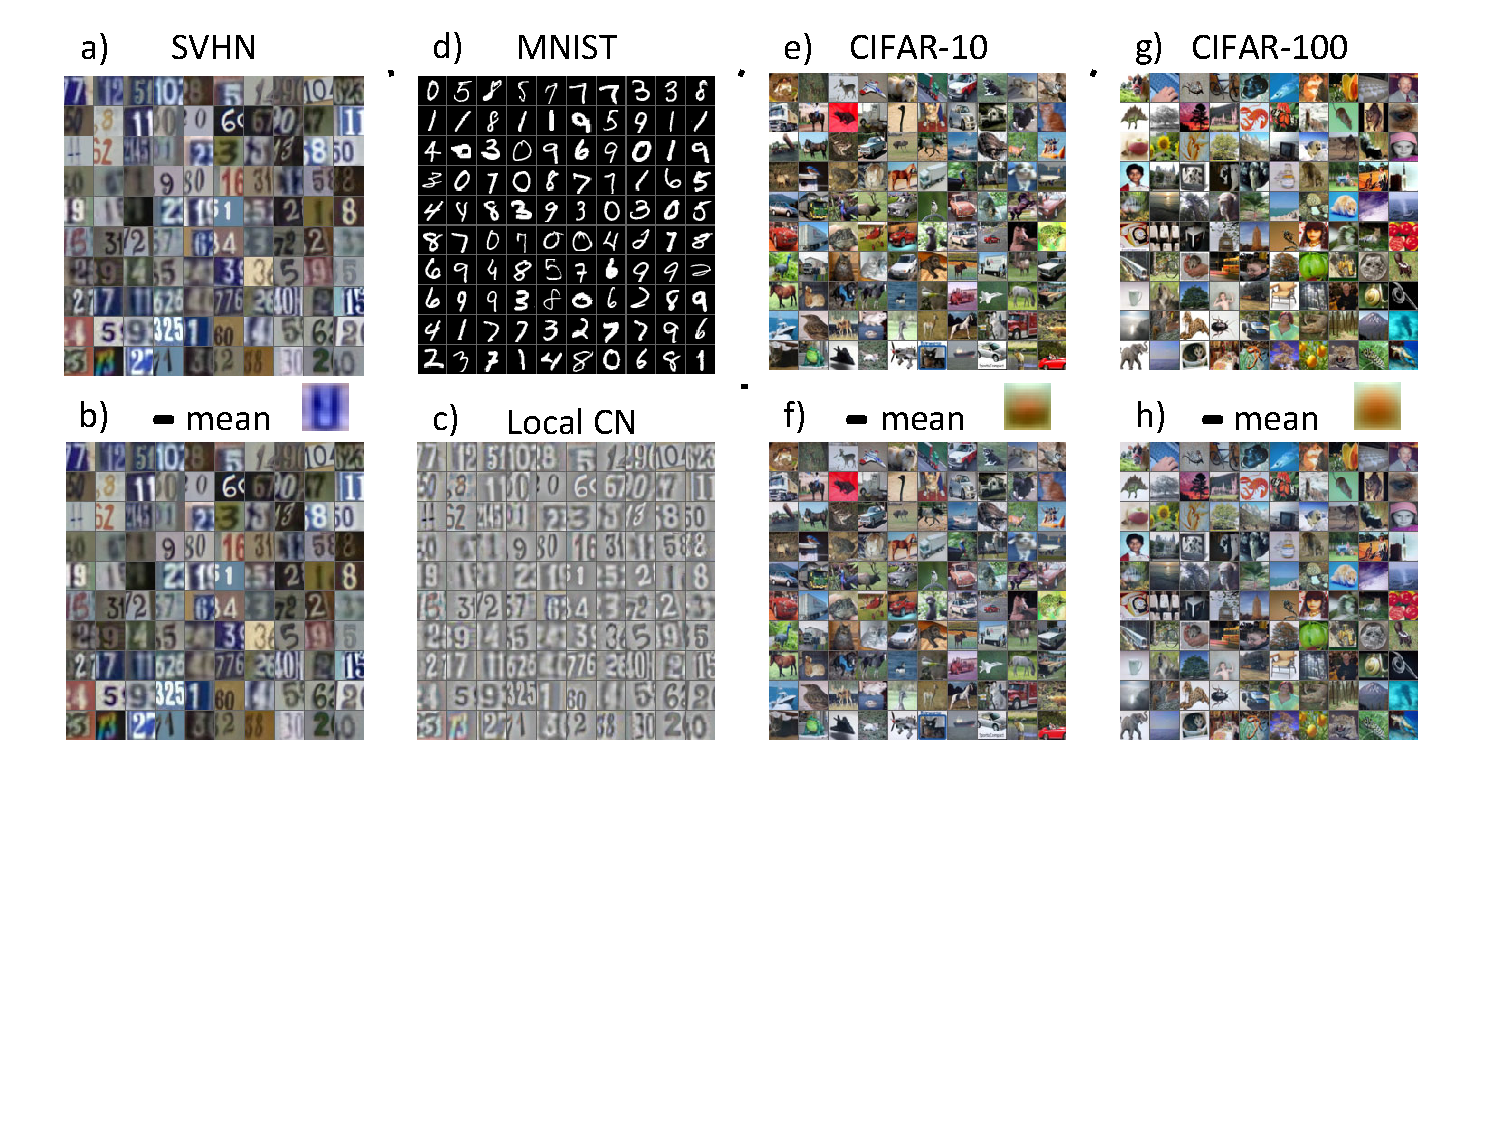
\includegraphics[width=5.5in]{datasets.pdf}
\end{center}
\vspace*{-0.4cm}
\caption{A selection of images from each of the datasets we
  evaluated. The top row shows the raw images while the bottom row are
  the preprocessed versions of the images we used for training. The
  CIFAR datasets (f,h) show slight changes by subtracting the per
  pixel mean, whereas SVHN (b) is almost indistinguishable from the
  original images. This prompted the use of local contrast
  normalization (c) to normalize the extreme brightness variations and
  color changes for SVHN.}
\label{fig:datasets}
\vspace*{-0.4cm}
\end{figure}

\subsection{CIFAR-10}
We begin our experiments with the CIFAR-10 dataset where
convolutional networks and methods such as dropout are known to work
well \cite{Hinton12,Kriz09}. This dataset is composed of 10 classes of
natural images with 50,000 training examples in total, 5,000 per
class. Each image is an RGB image of size 32x32 taken from the tiny
images dataset and labeled by hand. For this dataset we scale to [0,1] and follow Hinton \etal's \cite{Hinton12}
approach of subtracting the per-pixel mean computed over the dataset from each image as shown
in \fig{datasets}(f).

Cross-validating with a set of 5,000 CIFAR-10 training images, we
found a good value for the learning rate $\epsilon$ to be
$10^{-2}$ for convolutional layers and $1$ for the final softmax
output layer. These rates were annealed linearly throughout training
to $1/100th$ of their original values.
%This has the nice benefit of
%the user being able to set how long they're willing to run for and how
%much the learning rate should decrease by the end of training. Then
%all learning rates in the range are gradually utilized over the 280
%epochs we chose to run through the datasets.
Additionally, we found a small weight decay of $0.001$ to be optimal
and was applied to all layers. These hyper-parameter settings found through cross-validation were
used for all other datasets in our experiments.
%dded to convolutional and fully
%onnected weights helped. All these values were chosen using a
%alidation set for CIFAR-10, but worked well for all datasets in this
%aper.

Using the same network architecture described above, we trained
three models using average, max and stochastic pooling respectively and compare
their performance. \fig{cifar} shows the progression of train and test
errors over 280 training epochs. Stochastic pooling avoids
over-fitting, unlike average and max pooling, and produces less test
errors. \tab{cifar} compares the test performance of the three pooling
approaches to the current state-of-the-art result on CIFAR-10 which uses no data augmentation but
adds dropout on an additional locally connected layer
\cite{Hinton12}. Stochastic pooling surpasses this
result by 0.47\% using the same architecture but without requiring the
locally connected layer.



% We trained our convolutional network architecture with average pooling
% in each of the pooling layers, then again with max pooling, and again
% with stochastic pooling. In \fig{cifar} we plot the training and test
% error rates for classification throughout the 280 epochs of
% training. Notice how the training errors for max pooling quickly go to
% zero and the test errors plateau indicating drastic overfitting of the
% training set. Simpilarily the average pooling test error plateau at
% near the same performance. With stochastic pooling the error continue
% past either of the other methods and decrease througout training
% reaching a final result which to the best of our knowledge is state of
% the art for CIFAR-10 without any data augmentation \tab{cifar}.

\begin{figure}[t!]
\vspace*{-0.3cm}
\begin{center}
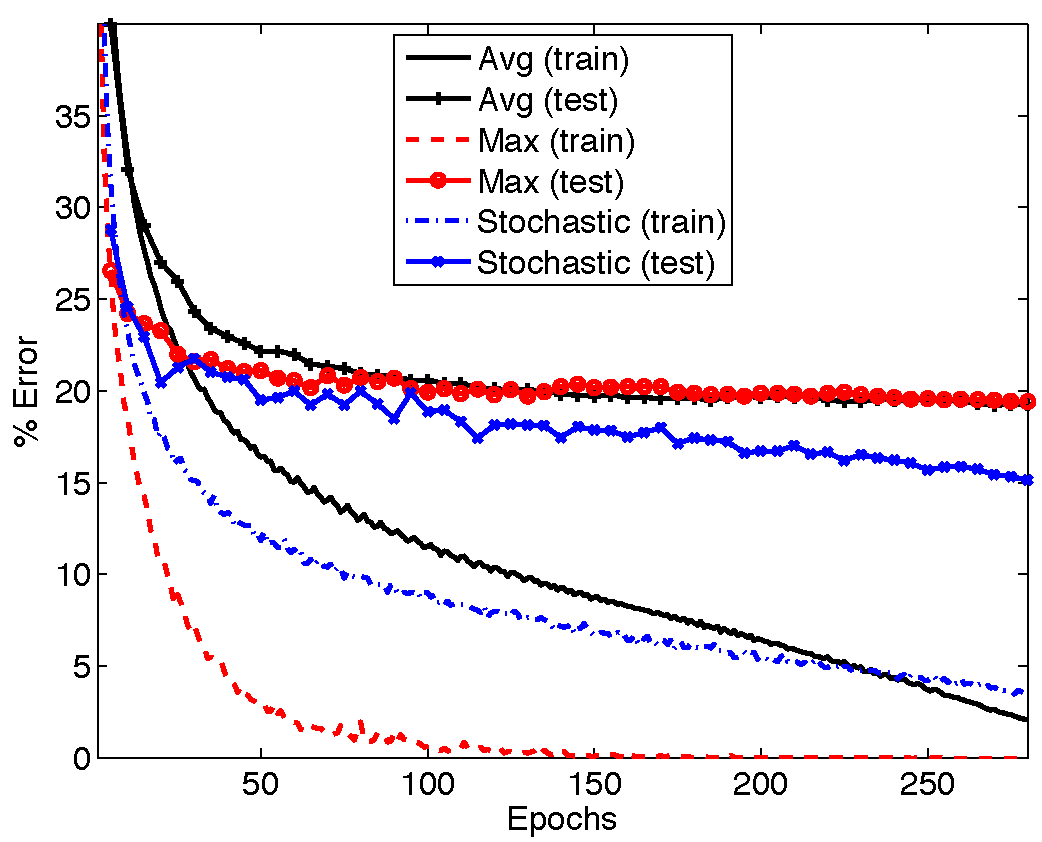
\includegraphics[width=2.8in]{CIFAR_errors.pdf}
\end{center}
\vspace*{-0.6cm}
\caption{CIFAR-10 train and test error rates throughout training for
  average, max, and stochastic pooling. Max and average pooling test
  errors plateau as those methods overfit. With stochastic pooling,
  training error remains higher while test errors continue to
  decrease.\footnotemark[1]}
\label{fig:cifar}
\vspace*{-0.3cm}
\end{figure}
\footnotetext[1]{Weight decay prevented training errors from reaching
  0 with average and stochastic pooling methods and required the high number
  of epochs for training. All methods performed slightly better with weight decay.}



%% FINAL
\begin{table}[h!]
\small
\vspace*{-2mm}
\begin{center}
\begin{tabular}{|l|c|c|}
  \hline
  & Train Error \% & Test Error \% \\
  \hline 3-layer Conv. Net  \cite{Hinton12} & -- & $16.6$ \\
  \hline 3-layer Conv. Net + 1 Locally Conn. layer with dropout \cite{Hinton12} & -- & $15.6$ \\
  \hline \hline % eid 91573
  Avg Pooling & $1.92$ & $19.24$ \\
   \hline % eid 91576
  Max Pooling & $0.0$ & $19.40$ \\
   \hline % eid 91579
  Stochastic Pooling & $3.40$ & $\textbf{15.13}$ \\
   \hline
\end{tabular}
\vspace*{-2mm}
\caption{CIFAR-10 Classification performance for various pooling
  methods in our model compared to the state-of-the-art performance
  \cite{Hinton12} with and without dropout.}
\label{tab:cifar}
\vspace*{-2mm}
\end{center}
\end{table}

To determine the effect of the pooling region size on the behavior of
the system with stochastic pooling, we compare the CIFAR-10 train
and test set performance for 5x5, 4x4, 3x3, and 2x2 pooling sizes
throughout the network in \fig{cifar_ps}. The optimal size appears to
be 3x3, with smaller regions over-fitting and larger regions possibly
being too noisy during training. At all sizes the stochastic pooling
outperforms both max and average pooling.


\begin{figure}[h!]
\begin{center}
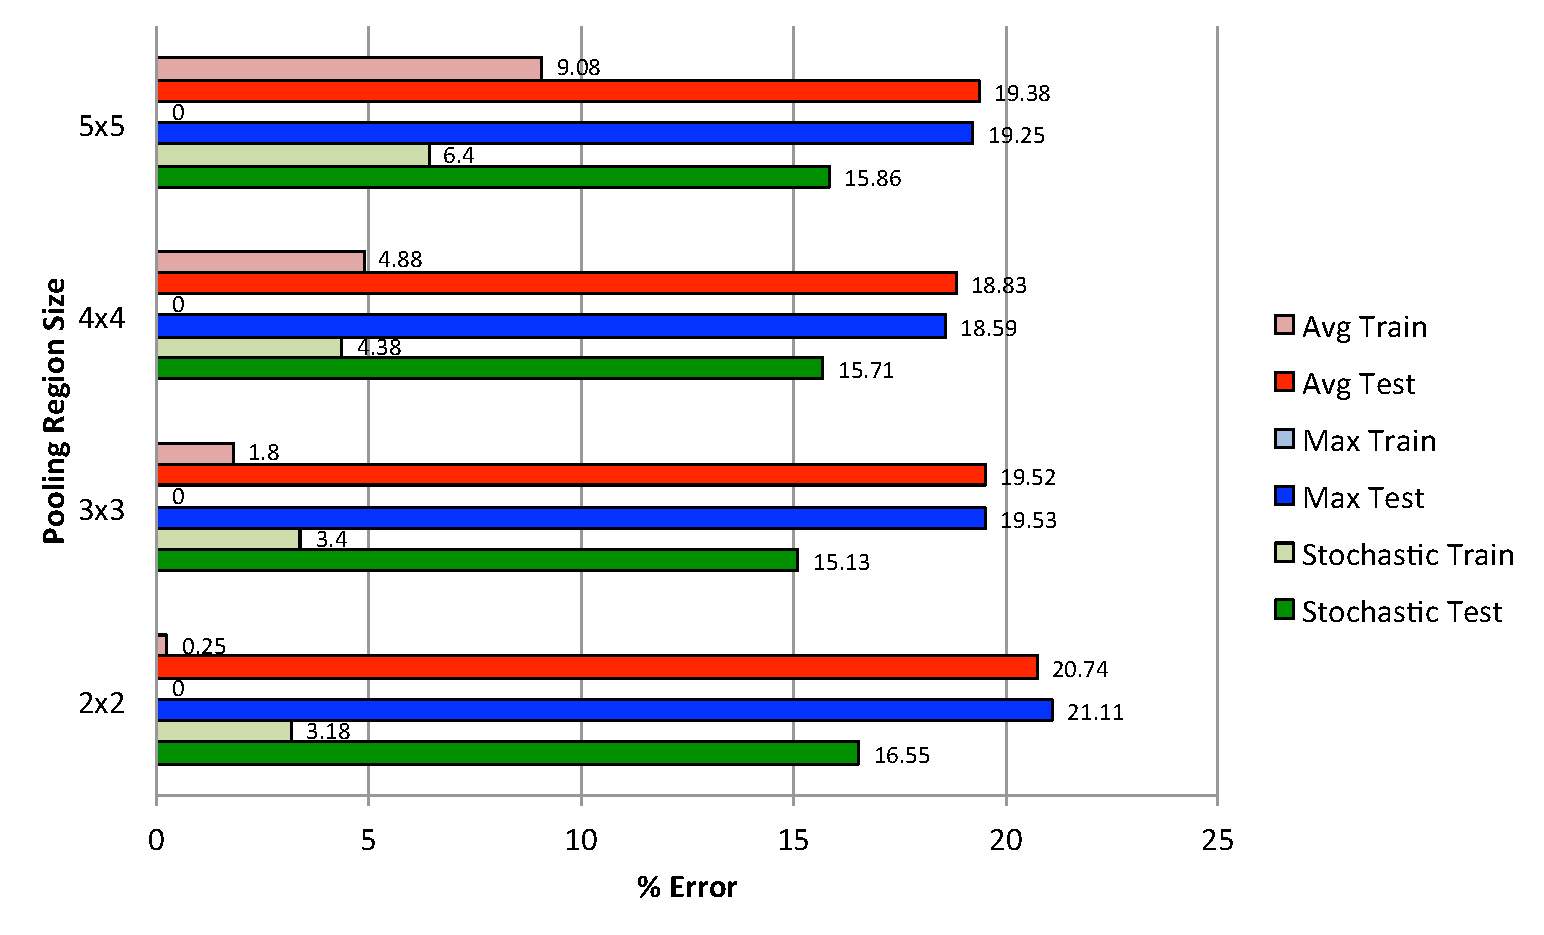
\includegraphics[width=4.8in]{psizes.pdf}
\end{center}
\vspace*{-0.8cm}
\caption{CIFAR-10 train and test error rates for various pooling region sizes with each method.}
\label{fig:cifar_ps}
\vspace*{-0.5cm}
\end{figure}



\subsection{MNIST}

The MNIST digit classification task is composed of 28x28 images of the
10 handwritten digits \cite{MNIST}. There are 60,000 training images with 10,000
test images in this benchmark. The images are scaled to [0,1] and we do not perform any other
pre-processing.

%% \begin{figure}[h!]
%% \begin{center}
%% \includegraphics[width=2.9in]{figs/MNIST_errors.pdf}
%% \end{center}
%% \vspace*{-0.3cm}
%% \caption{MNIST train/test error rates throughout training for average, max, and stochastic
%%   max pooling. Max pooling overfits the training set while average pooling is difficult to optimize
%%   and performs worse on the test set. Note: weight decay prevented training errors from
%%   reaching 0 in all methods.}
%% \label{fig:mnist}
%% \vspace*{-0.3cm}
%% \end{figure}

During training, the error using both stochastic pooling and max
pooling dropped quickly, but the latter completely overfit the
training data. Weight decay prevented average pooling from
over-fitting, but had an inferior performance to the other two
methods. \tab{mnist} compares the three pooling approaches to
state-of-the-art methods on MNIST, which also utilize convolutional
networks. Stochastic pooling outperforms all other methods that do not use
data augmentation methods such as jittering or elastic distortions \cite{mnistresults}.
The current state-of-the-art single model approach by Cireşan \etal
\cite{Ciresan11} uses elastic distortions to augment the
original training set. As stochastic pooling is a different type of
regularization, it could be combined with data augmentation to further
improve performance.

%   later in training. Average also did not overfit due
% to the weight decay, but performed inferior to both methods. Comparing
% this to state of the art methods on MNIST in \tab{mnist}, which also
% utilize convolutional networks, the stochastic pooling surpasses all
% other methods that do no use data augmentation methods such as
% jittering or elastic distortions. The work of Cireşan \etal
% \cite{Ciresan11} is the best single model on MNIST and utilizes
% elastic distortions to augment the original training set. Since our
% stochastic pooling is a different type of regularization, we could
% also leverage data augmentation to potentially improve performance.



%% FINAL
\begin{table}[h!]
\small
\vspace*{-2mm}
\begin{center}
\begin{tabular}{|l|c|c|}
  \hline
  & Train Error \% & Test Error \% \\
  \hline 2-layer Conv. Net + 2-layer Classifier  \cite{Jarrett2009} & -- & $0.53$ \\
  \hline 6-layer Conv. Net + 2-layer Classifier + elastic distortions \cite{Ciresan11} & -- & $0.35$ \\
  \hline  \hline   % eid 92142
  Avg Pooling & $0.57$ & $0.83$ \\
  \hline % eid 92143
  Max Pooling & $0.04$ & $0.55$ \\
  \hline % eid 92144
  Stochastic Pooling & $0.33$ & $\textbf{0.47}$ \\
  \hline
\end{tabular}
\vspace*{-2mm}
\caption{MNIST Classification performance for various pooling
  methods. Rows 1 \& 2 show the current state-of-the-art
  approaches.}
\label{tab:mnist}
\end{center}
\vspace*{-5mm}
\end{table}


\subsection{CIFAR-100}

The CIFAR-100 dataset is another subset of the tiny images dataset,
but with 100 classes \cite{Kriz09}. There are 50,000 training examples in total (500
per class) and 10,000 test examples. As with the CIFAR-10, we scale to [0,1] and subtract
the per-pixel mean from each image as shown in \fig{datasets}(h). Due
to the limited number of training examples per class, typical pooling
methods used in convolutional networks do not perform well, as shown in
\tab{cifar100}. Stochastic pooling outperforms these methods by
preventing over-fitting and surpasses what we believe to be the state-of-the-art
method by $2.66$\%.

%% FINAL
\begin{table}[h!]
\small
\vspace*{-2mm}
\begin{center}
\begin{tabular}{|l|c|c|}
  \hline
  & Train Error \% & Test Error \% \\
  \hline Receptive Field Learning \cite{Jia11} & -- & $45.17$ \\
  \hline  \hline   % eid 92258
  Avg Pooling & $11.20$ & $47.77$ \\
   \hline % eid 92259
  Max Pooling & $0.17$ & $50.90$ \\
   \hline % eid 92260
  Stochastic Pooling & $21.22$ & $\textbf{42.51}$ \\
   \hline
\end{tabular}
\vspace*{-1mm}
\caption{CIFAR-100 Classification performance for various pooling
  methods compared to the state-of-the-art method based on receptive
  field learning.}
\label{tab:cifar100}
\end{center}
\vspace*{-6mm}
\end{table}


\subsection{Street View House Numbers} \label{sec:SVHN}

The Street View House Numbers (SVHN) dataset is composed of 604,388
images (using both the difficult training set and simpler extra set)
and 26,032 test images \cite{SVHN}. The goal of this task is to classify the digit
in the center of each cropped 32x32 color image. This is a difficult real
world problem since multiple digits may be visible within each
image. The practical application of this is to classify house numbers
throughout Google's street view database of images.

We found that subtracting the per-pixel mean from each image did not
really modify the statistics of the images (see \fig{datasets}(b)) and
left large variations of brightness and color that could make
classification more difficult. Instead, we utilized local contrast
normalization  (as in \cite{Sermanet11}) on each of the three RGB channels to pre-process the
images \fig{datasets}(c). This normalized the brightness and color
variations and helped training proceed quickly on this relatively
large dataset.

Despite having significant amounts of training data, a large
convolutional network can still overfit. For this dataset, we train an additional model for 500
epochs with 64, 64 and 128 feature maps in layers 1, 2 and 3 respectively. Our stochastic pooling
helps to prevent overfitting even in this large model (denoted 64-64-128 in \tab{svhn}), despite
training for a long time. The existing
state-of-the-art on this dataset is the multi-stage
convolutional network of Sermanet \etal \cite{Sermanet11}, but
stochastic pooling beats this by $2.10$\% (relative gain of $43\%$).

%% STILL RUNNING
\begin{table}[h!]
\small
\vspace*{-2mm}
\begin{center}
\begin{tabular}{|l|c|c|}
  \hline
  & Train Error \% & Test Error \% \\
  \hline Multi-Stage Conv. Net + 2-layer Classifier  \cite{Sermanet11} & -- & $5.03$ \\
  \hline Multi-Stage Conv. Net + 2-layer Classifer + padding \cite{Sermanet11} & -- & $4.90$ \\
  \hline \hline   % eid 92246
  64-64-64 Avg Pooling  & $1.83$ & $3.98$ \\
  \hline % eid 92247
  64-64-64 Max Pooling  & $0.38$ & $3.65$ \\
  \hline % eid 92248
  64-64-64 Stochastic Pooling  & $1.72$ & $3.13$ \\ % Still waiting
  \hline \hline   % eid 92242
  64-64-128 Avg Pooling  & $1.65$ & $3.72$ \\
  \hline % eid 92243
  64-64-128 Max Pooling  & $0.13$ & $3.81$ \\
  \hline % eid 92244
  64-64-128 Stochastic Pooling  & $1.41$ & $\textbf{2.80}$ \\ % Still waiting
  \hline
\end{tabular}
\vspace*{-2mm}
\caption{SVHN Classification performance for various pooling methods in
  our model with 64 or 128 layer 3 feature maps compared to state-of-the-art results with and
  without data augmentation.}
\label{tab:svhn}
\vspace*{-6mm}
\end{center}
\end{table}


\subsection{Reduced Training Set Size}
\vspace{-1mm}
To further illustrate the ability of stochastic pooling to prevent
over-fitting, we reduced the training set size on MINST and CIFAR-10
datasets. \fig{reduced} shows test performance when training on a
random selection of only 1000, 2000, 3000, 5000, 10000, half, or the
full training set. In most cases, stochastic pooling overfits less than the other pooling
approaches.

\begin{figure}[h!]
\vspace*{-0.4cm}
\begin{center}
\mbox{
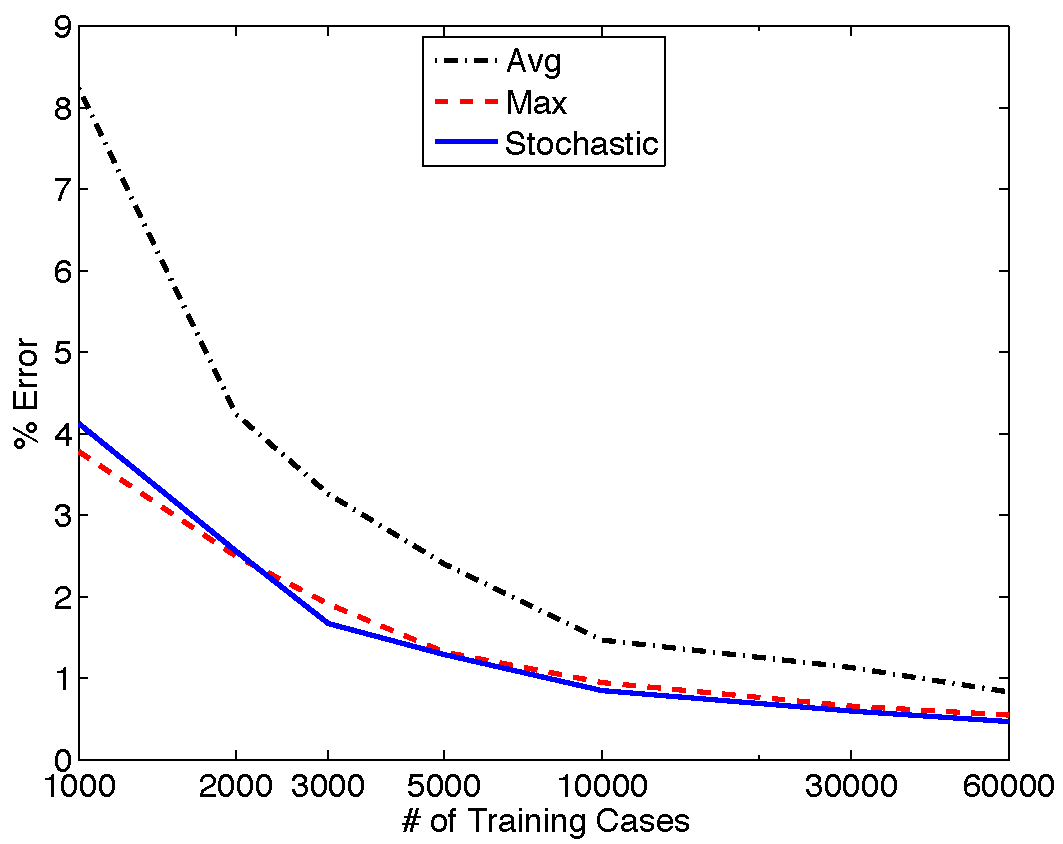
\includegraphics[width=2.5in]{MNIST_reduced.pdf}
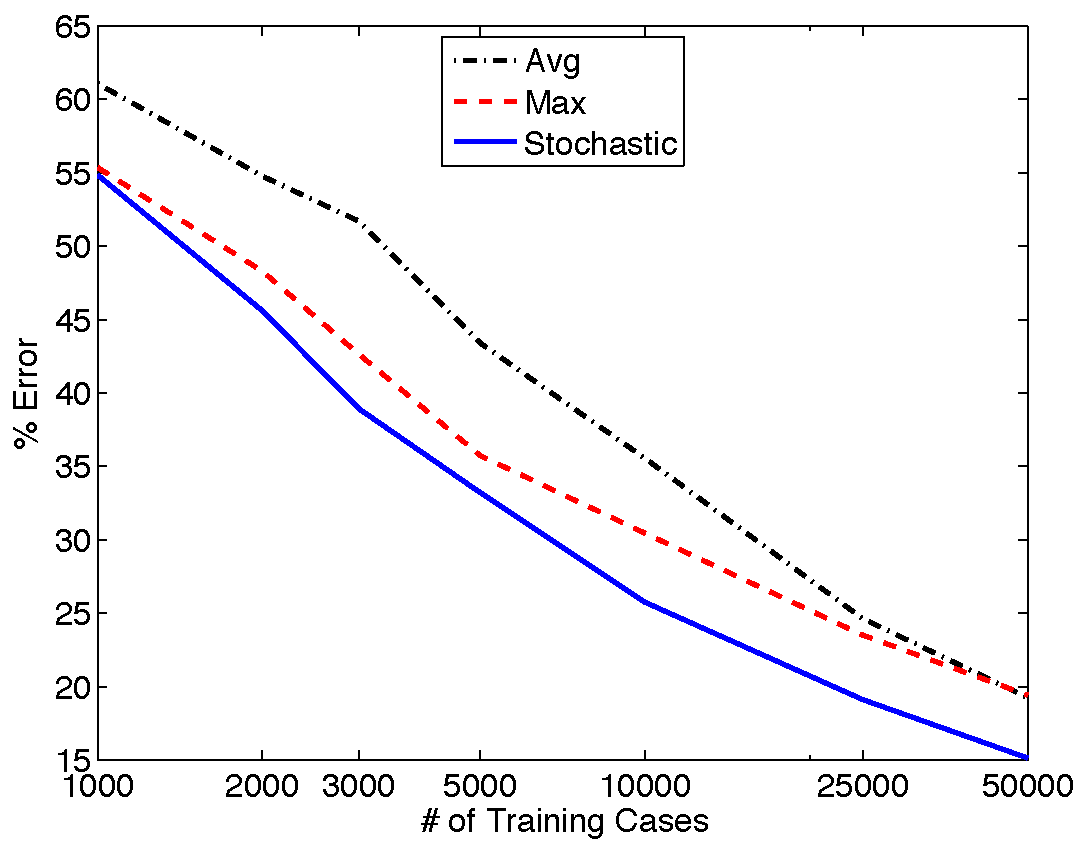
\includegraphics[width=2.5in]{CIFAR_reduced.pdf}}
\end{center}
\vspace*{-0.6cm}
\caption{Test error when training with reduced dataset sizes on MNIST (left) and
  CIFAR-10 (right). Stochastic pooling generally overfits the least. }
\label{fig:reduced}
\vspace*{-0.4cm}
\end{figure}


\subsection{Importance of Model Averaging} \label{sec:averaging}
\vspace{-1mm}
To analyze the importance of stochastic sampling at training time and
probability weighting at test time, we use different methods of
pooling when training and testing on CIFAR-10 (see
\tab{combos}). Choosing the locations stochastically at test time
degrades performance slightly as could be expected, however it still
outperforms models where max or average pooling are used at test
time. To confirm that probability weighting is a valid approximation to averaging many models, we draw $N$ samples
of the pooling locations throughout the network and average the output probabilities from those $N$
models (denoted Stochastic-$N$ in \tab{combos}). As $N$ increases, the results approach the
probability weighting method, but have the obvious downside of an $N$-fold increase in computations.

Using a model trained with max or average
pooling and using stochastic pooling at test time performs
poorly. This suggests that training with stochastic pooling, which
incorporates non-maximal elements and sampling noise, makes the model
more robust at test time. Furthermore, if these non-maximal elements
are not utilized correctly or the scale produced by the pooling
function is not correct, such as if average pooling is used at test
time, a drastic performance hit is seen.

When using probability weighting during training, the network easily
over-fits and performs sub-optimally at test time using any of the
pooling methods. However, the benefits of probability
weighting at test time are seen when the model has specifically
been trained to utilize it through either probability weighting or
stochastic pooling at training time.

\begin{table}[h!]
\small
\vspace*{-3mm}
\begin{center}
\begin{tabular}{|l|c|c|c|}
  \hline
  Train Method & Test Method & Train Error \% & Test Error \% \\
  \hline\hline
  Stochastic Pooling & Probability Weighting & $3.20$ & $\textbf{15.20}$ \\
   % eid 92425
  Stochastic Pooling & Stochastic Pooling & $3.20$ & $17.49$ \\
  Stochastic Pooling & Stochastic-10 Pooling & $3.20$ & $15.51$ \\
  Stochastic Pooling & Stochastic-100 Pooling & $3.20$ & $\textbf{15.12}$ \\
   % eid 92346
  Stochastic Pooling & Max Pooling & $3.20$ & $17.66$ \\ % done
   % eid 92409
  Stochastic Pooling & Avg Pooling & $3.20$ & $53.50$ \\ % done
  \hline\hline % eid 92349
  Probability Weighting & Probability Weighting & $0.0$ & $19.40$ \\
   % eid 92428
  Probability Weighting & Stochastic Pooling & $0.0$ & $24.00$ \\
   % eid 92353
  Probability Weighting & Max Pooling & $0.0$ & $22.45$ \\
   % eid 92430
  Probability Weighting & Avg Pooling & $0.0$ & $58.97$ \\
  \hline\hline % eid 92437
  Max Pooling & Max Pooling & $0.0$ & $19.40$ \\
  Max Pooling & Stochastic Pooling & $0.0$ & $32.75$ \\
  Max Pooling & Probability Weighting & $0.0$ & $30.00$ \\
  \hline\hline % eid 92439
  Avg Pooling & Avg Pooling & $1.92$ & $19.24$ \\
  Avg Pooling & Stochastic Pooling & $1.92$ & $44.25$ \\
  Avg Pooling & Probability Weighting & $1.92$ & $40.09$ \\
  \hline
\end{tabular}
\vspace*{-2mm}
\caption{CIFAR-10 Classification performance for various train and
  test combinations of pooling methods. The best performance is
  obtained by using stochastic pooling when training (to prevent
  over-fitting), while using the probability weighting at test time.}
\label{tab:combos}
\end{center}
\vspace*{-9mm}
\end{table}


\subsection{Visualizations}
\vspace{-2mm}
Some insight into the mechanism of stochastic pooling can be gained by using a deconvolutional
network of Zeiler \etal \cite{Zeiler11} to provide a novel visualization of our trained
convolutional network. The deconvolutional network has the same components (pooling, filtering) as a
convolutional network but are inverted to act as a top-down decoder that maps the top-layer feature
maps back to
the input pixels. The unpooling operation uses the stochastically chosen locations selected during
the forward pass. The deconvolution network filters (now applied to the feature maps, rather than
the input) are the transpose of the feed-forward filters, as in an auto-encoder with tied
encoder/decoder weights. We repeat this top-down process until the input pixel level is reached, producing
the visualizations in \fig{viscifar}. With max pooling, many of the input image edges are present,
but average pooling produces a reconstruction with no discernible structure.  \fig{viscifar}(a)
shows 16 examples of pixel-space reconstructions for different location samples throughout the
network. The reconstructions are similar to the max pooling case, but as the pooling locations
change they result in small local deformations of the visualized image.




%  The reconstructions using average pooling show no discernable
% structuer. With max pooling, the

% While the convolutional network was trained with no goal of
% reconstructing the input images, we can see from this visualization
% that much of structure from the images is preserved. This is not the
% case with average pooling.  Interestingly our projections down to
% pixel space resemble contrast normalized images in some aspects.


%  are shown. For
% each setting of the locations throughout the network we see how the
% network is potentially perceiving the input image.




% e
% deconvoltional network takes as input the top layer feature maps and
% projects down to the input image, unpooling

% Convolutional networks are typically viewed as black-boxes where an
% input image is mapped to an output label and little is know about how
% that mapping proceeds throughout the network. Recent work by Zeiler
% \etal \cite{Zeiler11} has shown interesting visualizations in terms of
% deconvolutional networks, essentially the inverse of convolutional
% networks. By tapping off the last layer of convolutional feature map
% activations of our CIFAR-10 model, we get what is similar to the
% inferred feature maps of a deconvolutional network. We use these to
% reconstruct downward through the network by unpooling through pooling
% layers using the location that was stochastically chosen in the
% feed-forward pass followed by convolving with the rotated filter
% templates in each convolution layer. Note, this process is similar to
% back-propagation through the network except the top level activations
% are used instead of gradients.
% We repeat this process until the pixel
% level is reached to produce the visualizations in
% \fig{viscifar}(a). Here we show 16 different samples of all the
% locations throughout the network are shown. For each setting of the
% locations throughout the network we see how the network is potentially
% perceiving the input image.

\begin{figure}[h!]
\vspace*{-0.3cm}
\begin{center}
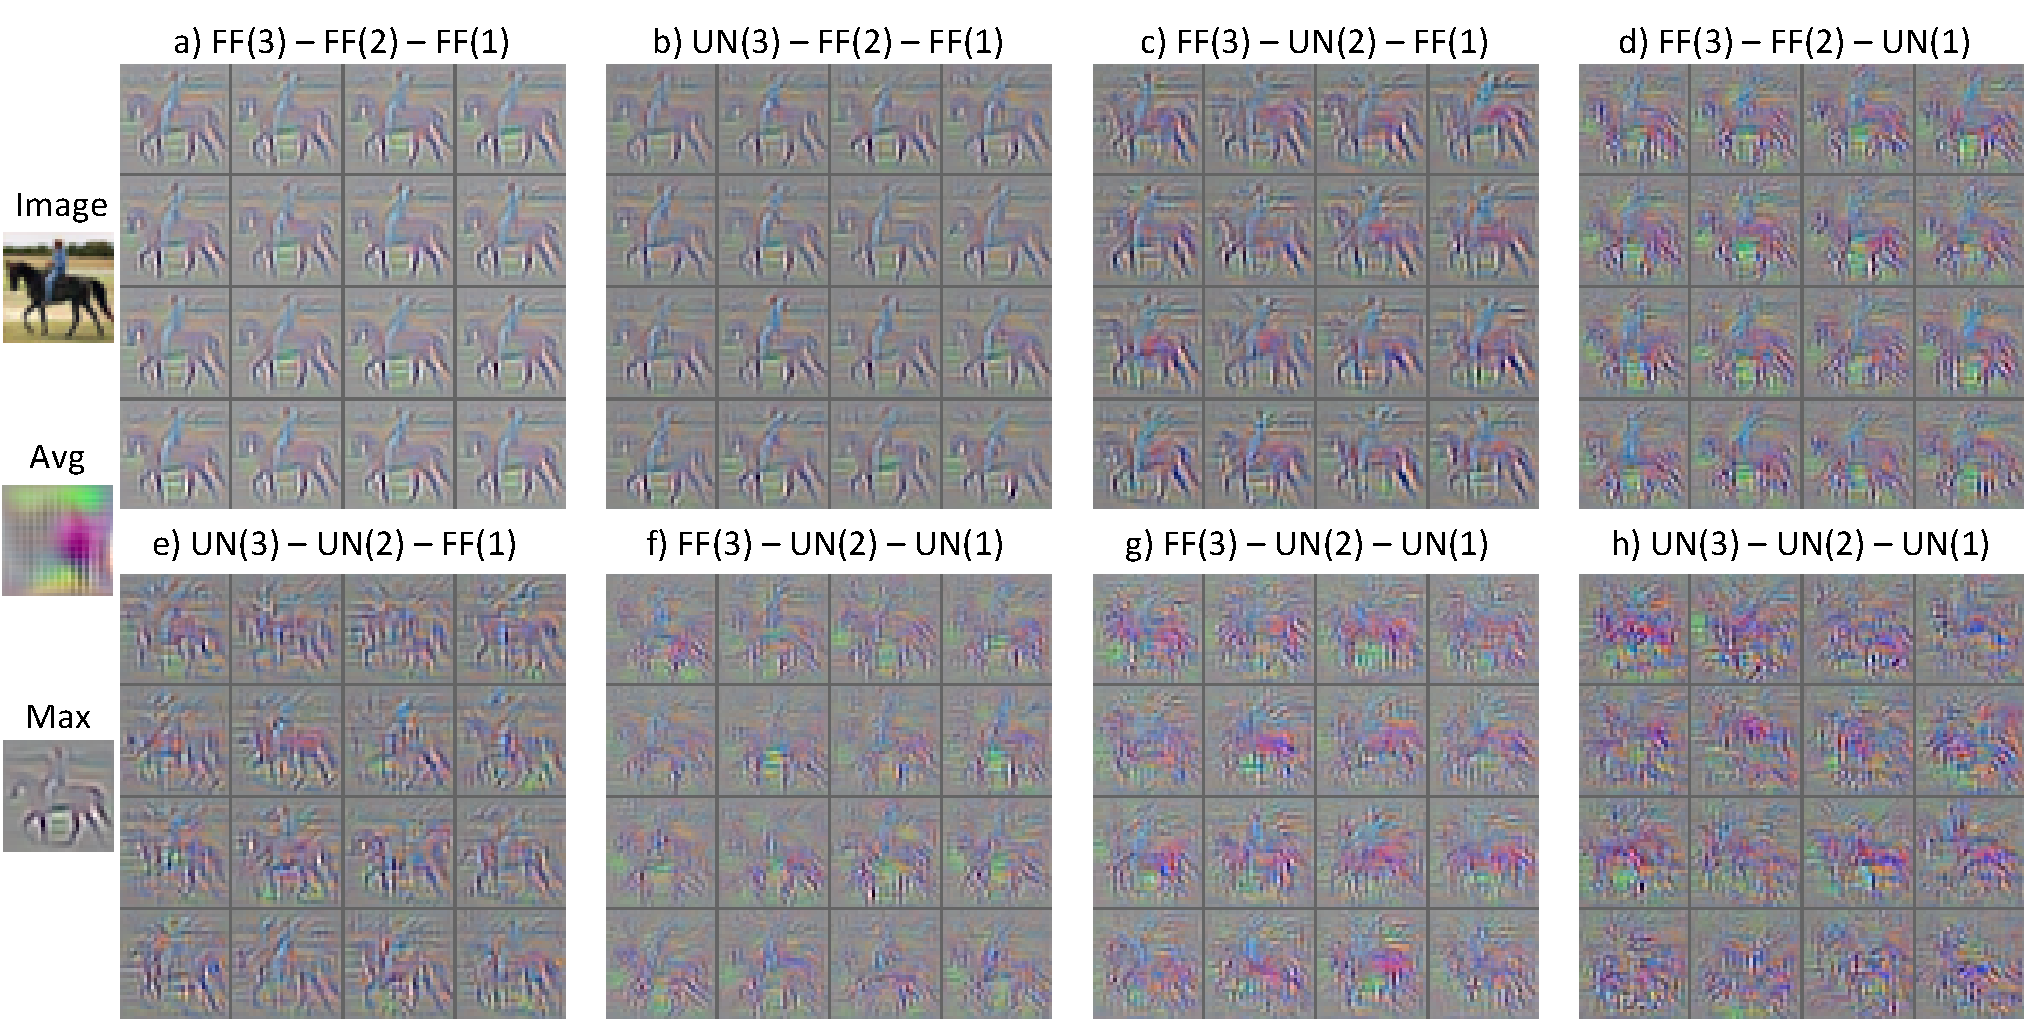
\includegraphics[width=5.5in]{vis.pdf}
\end{center}
\vspace*{-0.5cm}
\caption{Top down visualizations from the third layer feature map
  activations for the horse image (far left). Max and average pooling
  visualizations are also shown on the left. (a)--(h): Each image in a
  4x4 block is one instantiation of the pooling locations using
  stochastic pooling. For sampling the locations, each layer
  (indicated in parenthesis) can either use: (i) the multinomial
  distribution over a pooling region derived from the feed-forward
  (FF) activations as in \eqn{multinomial}, or (ii) a uniform (UN)
  distribution. We can see that the
  feed-forward probabilities encode much of the structure in the
  image, as almost all of it is lost when uniform sampling is used, especially in
  the lower layers. }
\label{fig:viscifar}
\vspace*{-3mm}
\end{figure}

Despite the stochastic nature of the model, the multinomial distributions
effectively capture the regularities of the data. To demonstrate this, we compare the outputs
produced by a deconvolutional network when sampling using the feedforward (FF) proabilities versus
sampling from uniform (UN) distributions.
In contrast to \fig{viscifar}(a) which uses only feedforward proabilities, \fig{viscifar}(b-h)
replace one or more of the pooling layers' distributions with uniform distributions.
The feed forward
probabilities encode significant structural information, especially in
the lower layers of the model.  Additional visualizations and videos of
the sampling process are provided as supplementary material at
\url{www.matthewzeiler.com/pubs/iclr2013/}.


% \fig{viscifar}(b-h) shows sampled locations using either the
% feed-forward probabilities (FF) used in our stochastic pooling or a
% uniform distribution (UN) over locations in a pooling region to
% exemplify the variability in the visualizations.


\vspace{-4mm}
\section{Discussion}
\vspace{-3mm}
We propose a simple and effective stochastic pooling
strategy that can be combined with any other forms of regularization
such as weight decay, dropout, data augmentation, etc.~to prevent
over-fitting when training deep convolutional networks. The method is
also intuitive, selecting from information the network is already
providing, as opposed to methods such as dropout which throw
information away. We show state-of-the-art performance on numerous
datasets, when comparing to other approaches that do not employ data
augmentation. Furthermore, our method has negligible computational
overhead and no hyper-parameters to tune, thus can be swapped into to
any existing convolutional network architecture.


%% References
\baselineskip=1pt
\bibliographystyle{plain}
\bibliography{iclr2013}
\end{document}
